\begin{figure}[htbp]
\centering 
  \subfloat[\acs{mus} = 0.1, spatial average.]
  {
	  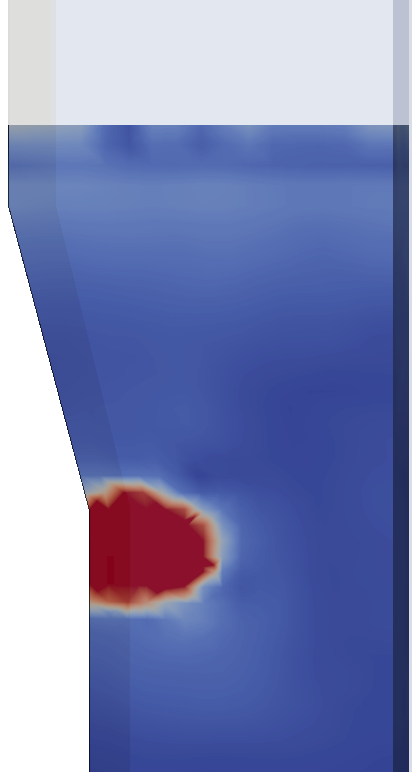
\includegraphics[width=.21\columnwidth]{images/291us_average_lf_stat}
	  \label{fig:291us_average_lf_stat}
  }
  \quad
    \subfloat[\acs{mus} = 0.1, velocity vectors.]
    {
	  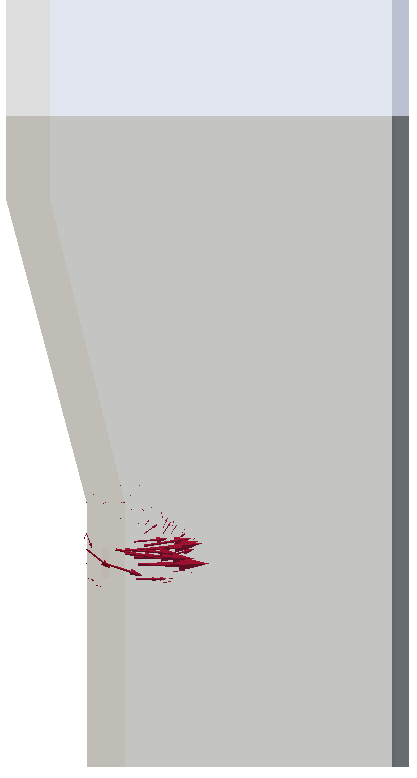
\includegraphics[width=.21\columnwidth]{images/290us_average_lf_arrow}
	  \label{fig:290us_average_lf_arrow}
  }
  \quad
    \subfloat[\acs{mus} = 0.1, stream lines.]
    {
	  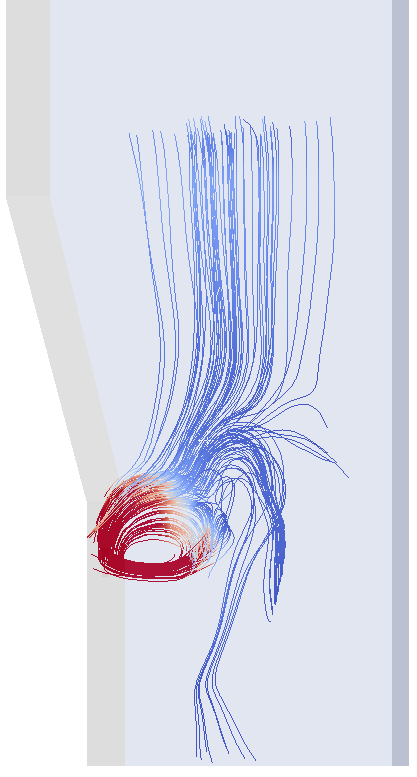
\includegraphics[width=.21\columnwidth]{images/292us_average_lf_stream}
	  \label{fig:292us_average_lf_stream}
  }
  \quad
  \subfloat[Legend.]
  {
	  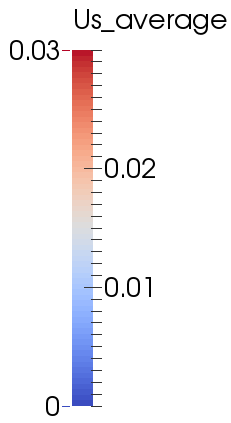
\includegraphics[width=.21\columnwidth]{images/278us_average_hf_legend}
	  \label{fig:278us_average_hf_legend}
  }
  \\
  \subfloat[\acs{mus} = 0.9, spatial average.]
  {
	  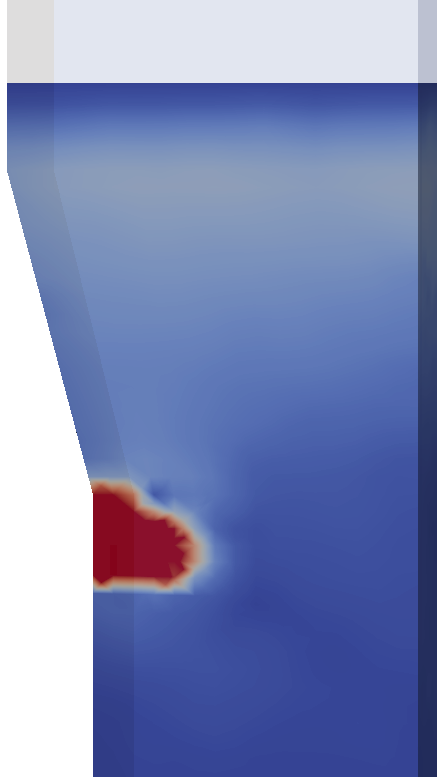
\includegraphics[width=.223\columnwidth]{images/280us_average_hf_stat}
	  \label{fig:280us_average_hf_stat}
  }
  \quad
    \subfloat[\acs{mus} = 0.9, velocity vectors.]
    {
	  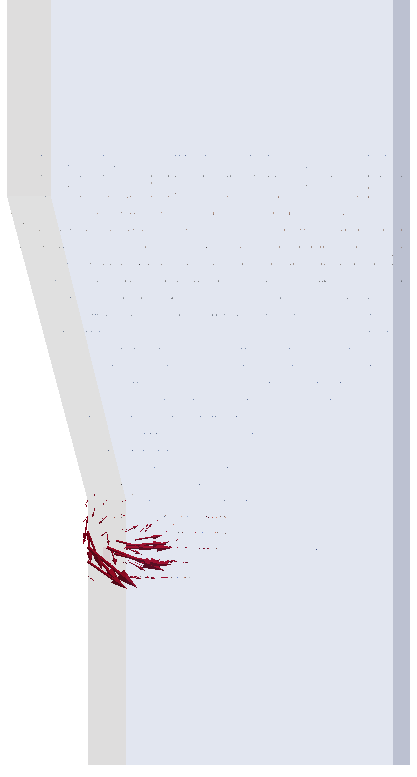
\includegraphics[width=.21\columnwidth]{images/279us_average_hf_arrow}
	  \label{fig:279us_average_hf_arrow}
  }
  \quad
    \subfloat[\acs{mus} = 0.9, stream lines.]
    {
	  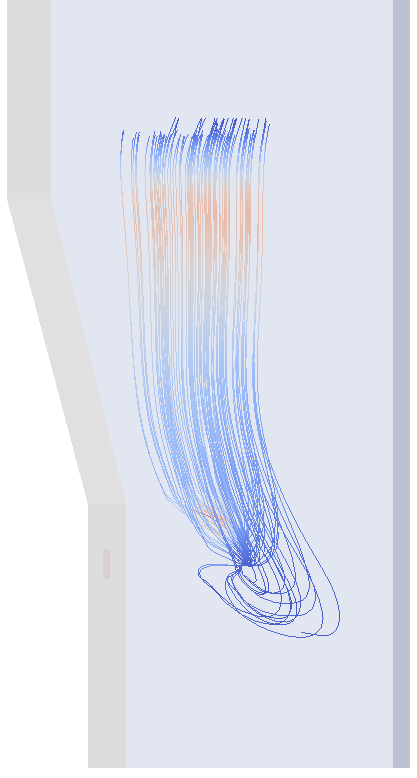
\includegraphics[width=.21\columnwidth]{images/281us_average_hf_stream}
	  \label{fig:281us_average_hf_stream}
  }
  \quad
  \subfloat[Legend.]
  {
	  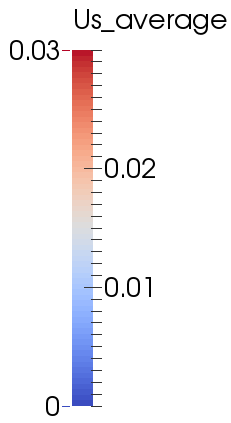
\includegraphics[width=.21\columnwidth]{images/278us_average_hf_legend}
	  \label{fig:278us_average_hf_legend}
  }
  \\  
  \caption[Vertical slice of particle velocity 1]{Vertical slice of fluid
  velocity 1. The effect of sliding friction over the particle velocity is
  consistent. The area with fast particles is almost 50\%
  larger in the low friction case.}
  \label{fig:300us_average_lf}
\end{figure}